\RequirePackage[l2tabu, orthodox]{nag}
\documentclass[version=3.21, pagesize, twoside=off, bibliography=totoc, DIV=calc, fontsize=12pt, a4paper]{scrartcl}
\input{preamble/packages}
\input{preamble/redac}
\input{preamble/math_basics}
%Pref
\NewDocumentCommand{\pref}{O{}}{⊳^{#1}}
\NewDocumentCommand{\prefeq}{O{}}{⊵^{#1}}
\NewDocumentCommand{\prefinv}{O{}}{⊲^{#1}}
\NewDocumentCommand{\prefeqinv}{O{}}{⊴^{#1}}
\NewDocumentCommand{\ppref}{}{\succ}
\NewDocumentCommand{\pprefeq}{}{\succeq}
\NewDocumentCommand{\pprefinv}{}{\prec}
\NewDocumentCommand{\pprefeqinv}{}{\preceq}
\NewDocumentCommand{\upb}{O{b}}{{\uparrow}#1}
\NewDocumentCommand{\downb}{O{b}}{{\downarrow}#1}
\NewDocumentCommand{\POs}{O{X}}{\mathit{PO}(#1)}

%Prob
\NewDocumentCommand{\inQ}{}{\intvl{1, \card{Q}}}
%Decision Theory (MCDA and SC)
\NewDocumentCommand{\allalts}{}{X}
\NewDocumentCommand{\allcrits}{}{\mathscr{C}}
\NewDocumentCommand{\alts}{}{A}
\NewDocumentCommand{\dm}{}{i}
\NewDocumentCommand{\allF}{}{\mathscr{F}}
\NewDocumentCommand{\allvoters}{}{\mathscr{N}}
\NewDocumentCommand{\voters}{}{N}
\NewDocumentCommand{\allprofs}{}{\bm{\mathcal{R}}}
\NewDocumentCommand{\prof}{}{\bm{R}}
\NewDocumentCommand{\linors}{O{X}}{\mathscr{L}(#1)}
%Thanks to https://tex.stackexchange.com/q/154549
	%\makeatletter
	%\def\@myRgood@#1#2{\mathrel{R^X_{#2}}}
	%\def\myRgood{\@ifnextchar_{\@myRgood@}{\mathrel{R^X}}}
	%\makeatother

%Deliberated Judgment
\NewDocumentCommand{\allargs}{}{S^*}
\NewDocumentCommand{\args}{}{S}
\NewDocumentCommand{\ar}{}{s}
\NewDocumentCommand{\allprops}{}{T}
\NewDocumentCommand{\prop}{}{t}
\NewDocumentCommand{\ileadsto}{}{⇝}
\NewDocumentCommand{\ibeatse}{}{⊳_\exists}
\NewDocumentCommand{\nibeatse}{}{⋫_\exists}
\NewDocumentCommand{\ibeatsst}{}{⊳_\forall}
\NewDocumentCommand{\nibeatsst}{}{⋫_\forall}
\NewDocumentCommand{\mleadsto}{O{\eta}}{⇝_{#1}}
\NewDocumentCommand{\mbeats}{O{\eta}}{⊳_{#1}}
\NewDocumentCommand{\ibeatseinv}{}{⊳_\exists^{-1}}

%Logic
\NewDocumentCommand{\ltru}{}{\texttt{T}}
\NewDocumentCommand{\lfal}{}{\texttt{F}}

\NewDocumentCommand{\relq}{}{\mathrel{?}}


\newcommand{\commentMP}[1]{\textcolor{green}{[MP:#1]}}
%I find these settings useful in draft mode. Should be removed for final versions.
	%Which line breaks are chosen: accept worse lines, therefore reducing risk of overfull lines. Default = 200.
		\tolerance=2000
	%Accept overfull hbox up to...
		\hfuzz=2cm
	%Reduces verbosity about the bad line breaks.
		\hbadness 5000
	%Reduces verbosity about the underful vboxes.
		\vbadness=1300

\title{Probabilistic elicitation of preferences \thanks{Draft!}}
\author{Nicolas Boria}
\author{Olivier Cailloux}
\author{Ararat Harutyunyan}
\affil{Université Paris-Dauphine, PSL Research University, CNRS, LAMSADE, 75016 PARIS, FRANCE\\
	\href{mailto:olivier.cailloux@dauphine.fr}{olivier.cailloux@dauphine.fr}
}

\begin{document}
\maketitle

\section{Introduction}
Many studies have investigated the computational complexity of (variants of) sorting problems. The usual implicit hypothesis is that the number of objects to be sorted is large, and that we are mostly interested in order of magnitudes of number of comparisons required to achieve some desired state of knowledge, rather than exact number of comparisons.

This article focuses on a different use case: obtaining preference information from an individual over a small set of objects. We assume furthermore that determining her preference among objects of the set is cognitively difficult for the individual. For example, one may be interested in determining (part of) someone’s preferences over a set of political candidates; or some juror “preferences” over competitors in some contest.

This problem can be viewed as a variant of a sorting task, where the ordering relation is the one determined by the individual’s preference. Querying for her preference is akin to a comparison in a sorting task. In such a setting, however, contrary to the implicit hypothesis in sorting tasks, it is important to focus on precise bounds on the number of comparisons, not just asymptotic orders of magnitude. This is for two reasons. First, the set of objects should generally be supposed to be small. That is because individuals will not accept to answer hundreds of comparison questions. Furthermore, when such comparison questions is cognitively difficult, a gain of a constant factor in terms of number of comparisons is important.

An example of an application of the sorts of results we seek is in social choice. In social choice, one typically assumes that the voters preferences are known, and studies focus on merits of aggregation rules. However, in many cases, the preferences must be elicited. A typical case is the one of a recrutment committee. Our results aim at indicating how to obtain (partial) information about the preferences of the members of the committee over the set of candidates. This can then be used, for example, to compute necessary or possible winner information.

\section{Set up and goal}
\begin{itemize}
	\item $\allalts$ a set of objects. Example: $\allalts = {a, b, c}$.
	\item $n = |\allalts|$. Example: $n = 3$.
	\item $\linors$ the set of linear orders over $\allalts$, that is, of transitive and complete binary relations over $\allalts$ (a relation $\prefeq$ over $\allalts$ is complete iff $\forall i, j \in \allalts: i \pref j \lor j \pref i$).
	\item ${\prefeq} \in \linors$ a preference over $\allalts$. Example: $\set{(a, b), (a, c), (b, c)}$. Let $\pref$ be the irreflexive part of $\prefeq$, thus, ${\prefeq} = ({\pref} \cup {=})$.
	\item Let $\powerset{S}$ denote the set of subsets of $S$.
Let $P: \powerset{\linors} → [0, 1]$ denote a probability distribution over the possible preferences.
\end{itemize}
The preference $\prefeq$ is a priori unknown.
We only know the probability distribution over $\linors$, from which $\prefeq$ is drawn. 
We can ask questions to obtain information about $\prefeq$. 
We are interested in comparing questioning strategies and in evaluating the probabilistic evolution of our knowledge of $\prefeq$ as a function of the number of questions asked, for various strategies. 

\section{Questioning to increase our knowledge}
Let $\POs$ denote the set of partial orders over $\allalts$. A partial order ${\pprefeq} \subseteq \allalts × \allalts$ is a transitive, reflexive and antisymmetric relation.
It represents our knowledge of $\pref$.
Let $\ppref$ be the irreflexive part of $\pprefeq$, thus, ${\pprefeq} = ({\ppref} \cup {=})$.

Let $\pprefeq_t$ denote our knowledge after $t$ questions (or $\ppref_t$ for its irreflexive part).
Define ${\ppref_0} = \emptyset$ as our (empty) knowledge after zero questions.
Example of $\ppref_1 : \set{(a, b)}$.

A question $q \in Q$ is a non-oriented edge, which formally we consider as two edges, inverse of each other. Let $q_{ij} = \set{(i, j), (j, i)}$ denote the question about ${i, j}$, with $i ≠ j \in \allalts$.
Note that $q_{ij} = q_{ji}$.
The set of possible questions is $Q = \set{q_{ij} \suchthat i ≠ j \in \allalts}$.
It follows that $\card{Q} = \binom{n}{2} = \frac{n (n - 1)}{2}$. In our running example, $\card{Q} = 3$.

Given $i ≠ j \in \allalts$, let $q_{ij}(\pref)$ represent, intuitively, the answer to the question $q_{ij}$ when the preference is $\pref$, that is, $q_{ij}(\pref)$ is the edge connecting $\set{i, j}$ that is in $\pref$, or formally, the element of the singleton ${\pref} \cap q_{ij}$.
Define an addition operation representing our increase in knowledge after having obtained an answer to a question: we add the resulting pair, and compute the transitive closure. Formally, given $\ppref$ and a question $q$, ${\ppref} + q(\pref) = T({\ppref} \cup \set{q(\pref)})$, where $T$ denotes the irreflexive transitive closure ($T(p) = \bigcup_{k \in N^*} p^k$). Example: $\set{(a, b)} + q_{bc}(\pref) = {\pref}$.

Let $K_\ppref = \set{\set{e, e^{-1}} \suchthat e \in {\ppref}} \subseteq Q$ denote the questions whose answer is known in $\ppref$. Note that $\card{K_\ppref} = \card{{\ppref}}$.
Let $Q_\ppref = Q \setminus K_\ppref$ denote the questions remaining given $\ppref$. Note that $\card{Q_\ppref} = \card{Q} - \card{K_\ppref}$.
Note that if we obtain at least one edge per step, then after $\card{Q}$ steps, our knowledge is complete: $Q_{\ppref_{\card{Q}}} = \emptyset$.

\subsection{Sequences of questions, of partial orders, and of digraphs}
There is a bijection between sequences of questions, sequences of partial orders, and sequences of digraphs.

Define the upper contour set of $x \in X$ as ${≥^{-1}}(x) = \set{y \in X \suchthat y ≥ x}$, thus, as the set of objects that are at least as good as $x$.
Towards showing the equivalence between a sequence of questions and a sequence of partial orders, we observe that a subset of an upper contour set that includes an object of which it is the upper contour set is the upper contour set of a unique object.
(A similar results holds for lower contour sets.)
\begin{proposition}[Folklore?]
	\label{th:ucs}
	Let $\set{x, y} \subseteq S \subseteq X$ such that $S \subseteq {≥^{-1}}(x)$ and $S \subseteq {≥^{-1}}(y)$. Then, $x = y$.
\end{proposition}
\begin{proof}
	By hypothesis, $x \in S$, and $\forall s \in S: s ≥ y$. Thus, $x ≥ y$.
	By a symmetrical observation, $y ≥ x$.
	Because $>$ is asymmetric and ${≥} = {>} \cup {=}$, this implies $x = y$.
\end{proof}

Given ${\ppref}, {\ppref'} \in \POs$ and $i, j \in \allalts$, say that the question $q_{ij} \in Q$ may lead from $\ppref$ to $\ppref'$ iff ${\ppref'} = {\ppref} + (i, j) \lor{\ppref'} = {\ppref} + (j, i)$.

Given ${\ppref}, {\ppref'} \in \POs$, say that the transition from $\ppref$ to $\ppref'$ is legal iff some question may lead from $\ppref$ to $\ppref'$.
Given $k \in \N$, let $\intvl{1, k}$ denote the interval of integers between $1$ and $k$.
Say that a sequence of partial orders $(\ppref_t) \in \POs^k$ is legal iff the transition from $\ppref_t$ to $\ppref_{t + 1}$ is legal $\forall t \in \intvl{1, k - 1}$.

Any legal sequence of partial orders defines uniquely a corresponding sequence of questions. The following proposition shows that any two adjacent partial orders in a legal sequence together define uniquely the left member of the answer that was added. As a similar result holds, by symmetry, for the right member, this proves the point.
\begin{proposition}
	Given ${\ppref}, {\ppref'} \in \POs$ and $i, j \in X$ such that ${\ppref'} = {\ppref} + (i, j)$, $i$ is determined uniquely by ${\ppref}$ and ${\ppref'}$.
\end{proposition}
\begin{proof}
	Let $N = {\ppref'} \setminus {\ppref}$ be the set of pairs brought thanks to the answer $(i, j)$. Suffices to prove that $N$ determine $i$ uniquely. 
	
	Consider $M = (N \cup {=})$, the reflexive relation equivalent to $N$.
	By definition of $+$, $M \subseteq \set{(i', j') \suchthat i' ≥ i \land j ≥ j'}$. 
	Let $L = M^{-1}(\allalts)$ be the left projection of $M$. 
	We see that $L$ includes $i$ and is a subset of the upper contour set of $i$. 
	\Cref{th:ucs} thus concludes.
\end{proof}

We can also think of $\ppref$ as a directed graph, or digraph, whose set of nodes is $\allalts$. We thus define a bijection that relates $\ppref$ to $G = (\allalts, \ppref)$, its corresponding digraph, and talk interchangeably about a digraph or a set of edges or a partial order. This bijection defines the possible digraphs: those having nodes $\allalts$ and a transitive and acyclic set of edges.

\section{Questioning strategies and probability distributions}
Define a questioning strategy as a function $s$ that given a current knowledge state ${\ppref} \in \POs$ returns a probability distribution over the set of possible questions $Q$. We write $P^\mathit{questions}(q \knowing {\ppref})$ for $s(\ppref)(q)$.

Define the probability of asking a sequence of questions $(q_t)_{t \in \N^*}$ when following the strategy $s$ and when the real preference is ${\prefeq} \in \linors$ as $P^s((q_t)_{t \in \N^*} \knowing {\prefeq}) = \prod_{t \in \N^*} P^\mathit{questions}((q_t \knowing {\pprefeq_{t - 1}})$, where ${\ppref_0} = \emptyset$ and ${\ppref_t} = {\ppref_{t - 1}} + q_t(\pref)$.

Together with the probability distribution $P$ over the possible preferences, this defines a joint probability distribution $P^s: \powerset{\linors × Q^{\N^*}} → [0, 1]$ over the possible preferences and questions asked, defined as $P^s(\pref, (q_t)_{t \in \N^*}) = P(\pref) P^s(q_t \knowing {\pref})$ (with an abuse of notation as we reuse the previously defined letter $P^s$ to define the joint probability distribution, which we can do as these usages coincide).
We also write $P$ instead of $P^\mathit{questions}$ as this introduces no ambiguity.

Thus, if $\card{Q} = 3$, $P^s(\pref, q_1, q_2, q_3)$ denotes the probability that the preference is $\pref$ and that the questions, chosen according to the strategy $s$, were $q_1$, then $q_2$, and finally $q_3$.
As the sequence of questions determines the sequence of partial orders, we can also consider $P^s$ as a probability distribution over sequences of partial orders. 
Example: $P^s({\ppref_1} = \set{(a, b)}) = P^s(q_1 = q_{ab} \land a \pref b)$.
Example: $P^s({\ppref_2} = \set{(a, b), (c, b)}) = P^s\big(\set{q_1, q_2} = \set{q_{ab}, q_{bc}} \land a \pref b \land c \pref b\big)$.

Define $P^\mathit{eq}$ as the equiprobable distribution over $\linors$, thus, $P^\mathit{eq}(\prefeq) = 1/\card{\linors}$.

Given $i, j \in \allalts$, $t \in \N$, define $P_t((i, j)) = P(i \ppref_t j)$ as the probability that the edge $(i, j)$ be known after $t$ questions.
Define $P_t(\set{i, j}) = P(q_{ij} \in K_{\ppref_t}) = 2 P_t(i > j)$ as the probability that the answer to the question about $\set{i, j}$ be known after $t$ questions.

Can we obtain a nice formula for $P_t(i, j)$?

\subsection{Random questions without repetition}
The random strategy without repetition draws a question, at each step, equiprobably from the set of remaining questions, or equiprobably from the set of possible questions if no question remain. Thus, $\forall {\ppref} \in \POs, i ≠ j \in \allalts$:
\begin{equation}
	P^\mathit{rd}(q_{ij} \knowing {\ppref}) = \left\{
	\begin{aligned}
		&\left.
		\begin{aligned}
			&\frac{1}{\card{Q} - \card{K_{\ppref}}} && \text{ if } q_{ij} \notin K_{\ppref}\\
			&\,0 && \text{ if } q_{ij} \in K_{\ppref}
		\end{aligned}\right\} && \text{ if } \card{K_{\ppref}} ≠ \card{Q},\\
		&\left.\frac{1}{\card{Q}}\right. && \text{ if } \card{K_{\ppref}} = \card{Q}.
	\end{aligned}\right.
\end{equation}

\subsection{Questioning by sorting a subset of objects}
Given a budget of $k$ questions, we can adopt the following questioning strategy. Fix $l$ objects such that they can be sorted by asking at most $k$ questions (thus $l$ greater than order of $\frac{k}{\log k}$?). Ask questions so as to sort them. We obtain $\card{{\ppref}} = \binom{l}{2}$.
Thus, perhaps, $\card{{\ppref}}$ is order of $\binom{k / \log k}{2}$.
TODO: be more precise.

\subsection{Median strategy}
(Thanks to Michail.)
Given a budget of $k$ questions, we can adopt the following questioning strategy. 
Fix $l$ objects.
Ask questions so as to: 1) determine their median in $\pref$ (“this can be done with O(l) comparisons deterministically”) and 2) partition the subset of $l$ objects among $\frac{l}{2}$ objects preferred to the median and $\frac{l}{2}$ other ones.
We obtain $\card{{\ppref}} = \frac{l^2}{4}$.
Thus, $\card{{\ppref}}$ order of $\frac{k^ 2}{4}$.
TODO: be more precise. See \hrefblue{https://en.wikipedia.org/wiki/Median_of_medians\#Proof_of_O(n)_running_time}{Median of medians}; Knuth, Sorting and Searching, vol. 3; Cormen, Intro to algorithms…

\section{The random strategy and equiprobable distribution}
Here we consider $P = P^\mathit{eq}$ and $s$ the random strategy without repetition. We also write $P$ instead of $P^s$.

\commentOC{We should rewrite this section to follow new notations and clarify (and continue)…}

When $\card{{\ppref_1}} = 1$, $P(\ppref_1) = \frac{1}{\card{Q}} \frac{1}{2}$.

Note that $P(\card{{\ppref_1}} = 1) = 1$, thus, $P(\ppref_2) = P(\ppref_2 \knowing \card{{\ppref_1}} = 1)$.

Let’s now evaluate $P(\ppref_2 \knowing \card{{\ppref_2}} = 2)$.
We may pick a question one end of which we know something about. There’s $2 (n - 2)$ such questions ($n - 2$ for each object in $\ppref_1$). If so, we need the answer to be oriented in a certain way to prevent transitive closure to bring anything new. Otherwise, we may pick a question whose two ends are yet unknown. There’s $n - 2$ choose $2$ such questions. Indeed, in total, there remains $2 (n - 2) + \frac{(n - 2) (n - 3)}{2} = \frac{(n - 2) (n + 1)}{2} = \frac{n (n - 1)}{2} - 1$ questions given $\ppref_1$.
Thus, $P(\ppref_2 \knowing \card{{\ppref_2}} = 2) = \frac{n - 1}{n + 1}$
(by noticing that $\card{Q_{\ppref_2}} = \frac{n(n-1)}{2}-1=\frac{(n-2)(n+1)}{2}$).

And $P(\ppref_2 \knowing \card{{\ppref_2}} = 3) = 2 \frac{2 (n - 2) 1/2}{(n - 2) (n + 1)} = \frac{2}{n + 1}$.

\section{Analysis for 4}
Taking a different starting point, say we may ask 3 questions and $n = 4$. Which questions should we ask to maximise the average number of resulting edges?
See \cref{fig:m4,fig:m4Cont}.

\begin{figure}
	\NewDocumentCommand{\pgfres}{}{\num[round-mode=places,round-precision=1]{\pgfmathresult}}
	\NewDocumentCommand{\pgfcalc}{m}{\pgfmathparse{#1}\num[round-mode=places,round-precision=1]{\pgfmathresult}}
	\NewDocumentCommand{\esp}{m}{E[.] = \pgfmathparse{#1}\num[round-mode=places,round-precision=1]{\pgfmathresult}}
	\begin{tikzpicture}
		\path (-10mm, -9mm) coordinate (offsetL);
		\path (10mm, -9mm) coordinate (offsetR);
		\path (0, -4mm) coordinate (offsetG);
		\path node (root0) {$a \relq b$, \esp{4}}
			[sibling distance = 6cm, level 2/.style = {sibling distance = 2cm}, level 3/.style = {sibling distance = 1cm}]
			child {
				node {$a > b$, \esp{4}}
				child[sibling distance = 3cm] {
					node {$b \relq c$, \esp{(4.5 * 4 + 5 * 2 + 3 * 6) / 12}}
					[sibling distance = 2cm]
					child[sibling distance = 2cm, align = left, anchor = north] {
						node {
							\tiny $a > b > c$, \esp{4.5}\\
							$dabc$\\
							$adbc$\\
							$abdc$\\
							$abcd$
						}
					}
					child[sibling distance = 2cm, align = left, anchor = north] {
						node {
							$\set{a, c} > b$, \esp{(5 * 2 + 3 * 6) / 8}\\
							$cab$ × 4\\
							$acb$ × 4
						}
					}
				}
				child {
					node {$c \relq d$, \esp{4}}
					child {
						node {…}
					}
					child {
						node {…}
					}
				}
				child[sibling distance = 1.5cm] {
					node {…}
				}
			}
			child {
				node {$b > a$}
				child[sibling distance = 3cm] {
					node {$b \relq c$}
					child[sibling distance = 2cm] {
						node {$b > \set{a, c}$}
					}
					child[sibling distance = 2cm] {
						node {$c > b > a$}
					}
				}
				child {
					node {$b \relq d$}
					child {
						node {…}
					}
					child {
						node {…}
					}
				}
				child[sibling distance = 1.5cm] {
					node {…}
				}
			}
		;
		\path node[fit = (root0) (root0-1-1.south west) (root0-2-3.south east) (root0-2-2-2.south east)] (tree0) {};
		
		\path (tree0.south) ++ (0, -1cm) node[anchor = north] (root abc) {$a > b > c$, \esp{4.5}}
			[sibling distance = 4cm, level 2/.style = {sibling distance = 2cm, align = left, anchor = north}]
			child {
				node {$c \relq d$, \esp{(6 * 1 + 4 * 3) / 4}}
				child {
					node {
						6 edges\\
						$abcd$
					}
				}
				child {
					node {
						4 edges\\
						$abdc$\\
						$adbc$\\
						$dabc$
					}
				}
			}
			child {
				node {$b \relq d$, \esp{4}}
				child {
					node {
						4 edges\\
						$abcd$\\
						$abdc$
					}
				}
				child {
					node {
						4 edges\\
						$adbc$\\
						$dabc$
					}
				}
			}
			child {
				node {$a \relq d$, \esp{(6 * 1 + 4 * 3) / 4}}
				child {
					node {
						4 edges\\
						$adbc$\\
						$abdc$\\
						$abcd$
					}
				}
				child {
					node {
						6 edges\\
						$dabc$
					}
				}
			}
		;
		\begin{scope}
			\path[anchor=base] (root abc-1) ++ (offsetL) ++ (0mm, 7mm) node (a) {$a$} ++(offsetG) node (b) {$b$} ++(offsetG) node (c) {$c$} ++ (offsetG) node (d) {$d$};
			\path graph[use existing nodes] {a -- b -- c -- d};
		\end{scope}
		\begin{scope}
			\path (0, -6mm) coordinate (offsetG);
			\path[anchor=base] (root abc-1) ++ (offsetR) ++ (-1mm, 6mm) node (a) {$a$} ++(offsetG) node (b) {$b$} ++(offsetG) node (c) {$c$} ++(3mm, 6mm) node (d) {$d$};
			\path graph[use existing nodes] {a -- b -- c -- d};
		\end{scope}

		\path (root abc) ++ (0, -5.5cm) [sibling distance = 3cm, level 2/.style = {sibling distance = 1.5cm, align = left, anchor = north}] node[anchor=north] (root ac b) {$\set{a, c} > b$, \esp{(5 * 2 + 3 * 6) / 8}}
			child {
				node {$a \relq c$, \esp{3}}
				child {
					node {
						3 edges\\
						$dacb$\\
						$adcb$\\
						$acdb$\\
						$acbd$
					}
				}
				child {
					node {
						3 edges\\
						$dcab$\\
						$cdab$\\
						$cadb$\\
						$cabd$
					}
				}
			}
			child {
				node {$a \relq d$, \esp{(3 * 5 + 4 * 3) / 8}}
				child {
					node {
						3 edges\\
						$adcb$\\
						$acdb$\\
						$acbd$\\
						$cadb$\\
						$cabd$
					}
				}
				child {
					node {
						4 edges\\
						$cdab$\\
						$dcab$\\
						$dacb$
					}
				}
			}
			child {
				node {$b \relq d$, \esp{(5 * 2 + 3 * 6) / 8}}
				child {
					node {
						5 edges\\
						$cabd$\\
						$acbd$
					}
				}
				child {
					node {
						3 edges\\
						$acdb$\\
						$adcb$\\
						$cadb$\\
						$cdab$\\
						$dacb$\\
						$dcab$
					}
				}
			}
		;
%		\begin{scope}
%			\path (0, -8mm) coordinate (offsetG);
%			\path[anchor=base] (root ac b-3) ++ (offsetL) ++ (-1mm, 4mm) node (a) {$a$} ++(offsetG) node (b) {$b$} ++(3mm, 8mm) node (c) {$c$} ++(offsetG) node (d) {$d$};
%			\path graph[use existing nodes] {a -- b -- c -- d};
%		\end{scope}
%		\begin{scope}
%			\path (0, -7mm) coordinate (offsetG);
%			\path[anchor=base] (root ac b-3) ++ (offsetR) ++ (-2mm, 2mm) node (a) {$a$} ++(offsetG) node (b) {$b$} ++(3mm, 7mm) node (c) {$c$} ++(0, 6mm) node (d) {$d$};
%			\path graph[use existing nodes] {a -- b -- c -- d};
%		\end{scope}
%		\begin{scope}
%			\path (0, -5mm) coordinate (offsetG);
%			\path[anchor=base] (root ac b-4) ++ (offsetL) ++ (2mm, 3mm) node (a) {$a$} ++(offsetG) node (b) {$b$} +(3mm, 5mm) node (c) {$c$} ++(offsetG) node (d) {$d$};
%			\path graph[use existing nodes] {a -- b -- {c, d}};
%		\end{scope}
%		\begin{scope}
%			\path (0, -5mm) coordinate (offsetG);
%			\path[anchor=base] (root ac b-4) ++ (offsetR) ++ (-1mm, 3mm) node (a) {$a$} ++(offsetG) node (b) {$b$} +(3mm, 5mm) node (c) {$c$} ++(-3mm, 5mm) node (d) {$d$};
%			\path graph[use existing nodes] {a -- b -- {c, d}};
%		\end{scope}
	\end{tikzpicture}
	\caption{The case $m = 4$, three questions.}
	\label{fig:m4}
\end{figure}

\begin{figure}
	\NewDocumentCommand{\pgfres}{}{\num[round-mode=places,round-precision=1]{\pgfmathresult}}
	\NewDocumentCommand{\pgfcalc}{m}{\pgfmathparse{#1}\num[round-mode=places,round-precision=1]{\pgfmathresult}}
	\NewDocumentCommand{\esp}{m}{E[.] = \pgfmathparse{#1}\num[round-mode=places,round-precision=1]{\pgfmathresult}}
	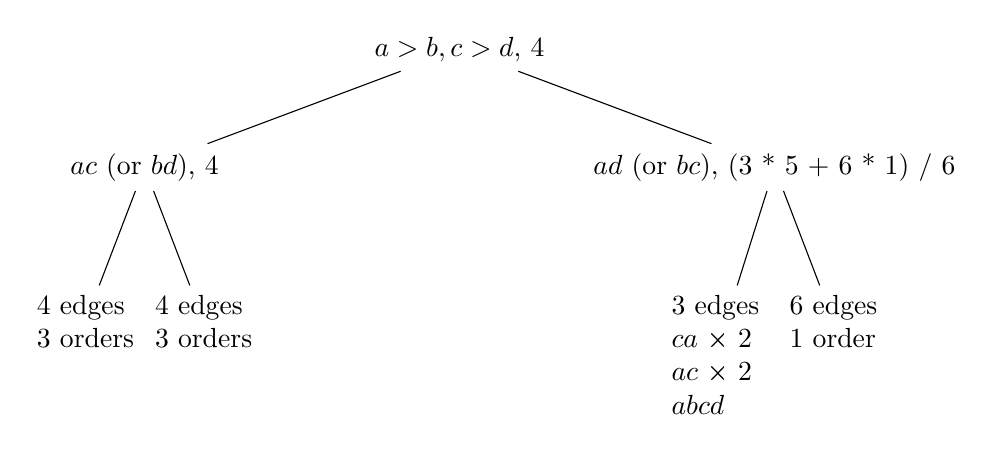
\begin{tikzpicture}
		\path (-10mm, -9mm) coordinate (offsetL);
		\path (10mm, -9mm) coordinate (offsetR);
		\path (0, -4mm) coordinate (offsetG);
		\path [sibling distance = 8cm, level 2/.style = {sibling distance = 1.5cm, align = left, anchor = north}] node[anchor=north] {$a > b, c > d$, \esp{4}}
			child {
				node {$a \relq c$ (or $b \relq d$), \esp{4}}
				child {
					node {
						4 edges\\
						3 orders
					}
				}
				child {
					node {
						4 edges\\
						3 orders
					}
				}
			}
			child {
				node {$a \relq d$ (or $b \relq c$), \esp{(3 * 5 + 6 * 1) / 6}}
				child {
					node {
						3 edges\\
						$ca$ × 2\\
						$ac$ × 2\\
						$abcd$
					}
				}
				child {
					node {
						6 edges\\
						1 order
					}
				}
			}
		;
	\end{tikzpicture}
	\caption{The case $m = 4$, three questions, continued.}
	\label{fig:m4Cont}
\end{figure}

%\bibliography{bibl}

\appendix
\section{Best possible number of edges}
Assume we are the luckiest possible: we can choose the orientation of edges (the answers to questions) so as to maximise the number of resulting edges.

Define the \emph{original graph} as the graph $G$ containing the edge $(a, b)$ iff the question $a \relq b$ was asked and answered with $a > b$. Consider $k < n$. After $k$ questions, $G$ has $k$ edges at best.
The following proposition shows that to maximise the number of edges, it is necessary and sufficient to choose any $k + 1$ vertices and connect them. Note that any graph $G$ with $k$ edges can be uniquely decomposed into components having $k_1$, $k_2$, … edges, with $\sum_i k_i = k$ (in a component, there is a non-oriented path linking any two vertices of the component, and any two components are disconnected).
\begin{proposition}
	Let $G = (\allalts, E)$ be an oriented acyclic graph (not necessarily closed transitively) composed of components having $k_1$, $k_2$, … edges, with $\sum_i k_i = k$.
	Then, its transitive closure $T_G$ has $\binom{k + 1}{2}$ edges iff there is only one component having $k$ edges; otherwise, $T_G$ has less than $\binom{k + 1}{2}$ edges.
\end{proposition}
\begin{proof}[Folklore?]
	In general, $T_G$ has at most $\sum_i \binom{k_i + 1}{2}$ edges. The claim holds because $\binom{k + 1}{2} ≥ \sum_i \binom{k_i + 1}{2}$, with equality iff there is only one component.
	Indeed, the left hand side is half of $(k + 1) k = (\sum_i k_i + 1) \sum_i k_i = (\sum_i k_i)^2 + \sum_i k_i ≥ \sum_i k_i^2 + \sum_i k_i$, with equality iff there is only one component; whereas the right hand side is half of $\sum_i (k_i + 1) k_i = \sum_i k_i^2 + \sum_i k_i$.
\end{proof}

\section{Example context}
$N$ the voters (reviewers), $\card{N} = n$; $X$ the items (articles submitted to a conference), $\card{X} = m$. $PO(X)$ the partially ordered sets over $X$. Let $Q \in PO(X)^N$ represent some partial knowledge of the voters preferences. Consider $f: PO(X)^N → \powersetz{X}$ an enlarged voting rule, that selects winning items on the basis of partial knowledge of the preferences of the voters. Define $f(Q) = \min_{x \in X} \max_{y \in X, (>_{i \in N}) \in compl(Q)} s(y, (>_{i \in N})) - s(x, (>_{i \in N}))$ as selecting the alternatives that minimize the worst regret, where $s$ is the Borda scoring rule (attributing to an alternative at a profile as many points as that alternative beats other alternatives, summed over all voters).

We are interested in asking questions so as to let the regret diminish as fast as possible.
\end{document}

